\chapter{Introduction}\label{chap:introduction}
\subsection{Galaxy}
Galaxy {\footnote{\url{https://usegalaxy.eu/}}} is an open-source biological data processing and research platform. It supports numerous types of extensively used biological data formats like FASTA, FASTAQ, GFF, PDB and many more. To process these datasets, Galaxy offers tools and workflows which either transform these datasets from one type to another or manipulate the data. A simple example of data processing is to merge two compatible datasets to make one. Another example can be to reverse complement a sequence of nucleotides. \footnote{\url{https://usegalaxy.eu/?tool_id=MAF_Reverse_Complement_1&version=1.0.1&__identifer=zmk9dx9ivbk}}

\begin{figure}[h]
\begin{centering}
    {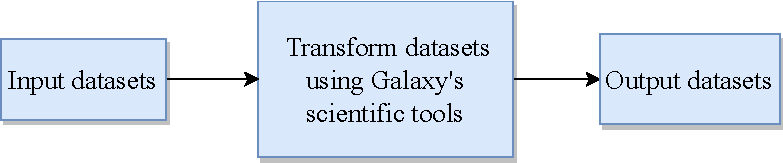
\includegraphics[scale=0.8]{figures/image_Galaxy_1.pdf}}
    \caption[Galaxy tools and workflows]{\textbf{Galaxy tools and workflows} This images shows the basic form in which tools and workflows carry out a task}
    %\label{fig:pcaclasses}
\end{centering}
\end{figure}

A tool is a data-transforming entity which allows one or more types of datasets, transforms these datasets and releases output datasets in one or more types.


The workflows are data processing pipelines. A set of tools joined one after another constitute a workflow. A workflow can have one or more starting and ending tools. The tools which are connected 



\subsection{Galaxy tools}

\subsection{Tool categories}

\subsection{Motivation}
